\section{一个有趣的应用:匿名路由}\label{sec:2-4}

我们的老朋友 Alice 想向 Bob 发送一条消息 $m$,但她不想让 Bob 或其他人知道这条消息 $m$ 是来自 Alice 的。比如说,Bob 可能在经营一个公共论坛,而 Alice 想在论坛上匿名发布一条评论。匿名发帖可以让 Alice 在不表明自己的真实身份的前提下自由地讨论健康问题,或者任何其他可能会定位到她个人的敏感议题。在本节中,我们假设 Alice 只想在论坛上发布\emph{一条}消息。

一种方法是,Alice 选择一个代理 Carol,将 $m$ 发送给 Carol,并让 Carol 将消息转发给 Bob。这显然不能为 Alice 提供匿名性,因为任何监测网络的人都能看到 $m$ 是由 Alice 发给 Carol,再由 Carol 发给 Bob 的。通过追踪 $m$ 在网络中的路径,任何人都可以看到这个帖子来自于 Alice。

一种更好的方法是,Alice 与 Carol 建立一个共享密钥 $k$,并向 Carol 发送 $c:=E(k,m)$,其中 $\mathcal{E}=(E,D)$ 是一个语义安全的密码。Carol 对 $c$ 进行解密,并将 $m$ 转发给 Bob。现在,监测网络的人将看到一条由 Alice 发给 Carol 的消息,以及另一条由 Carol 发给 Bob 的消息。然而,这种方法仍然不能确保 Alice 的匿名性:如果在某一天,Carol 收到的唯一消息就来自 Alice,而她发送的唯一消息是给 Bob 的,那么监测者就可以将这两者联系起来,并推断发布的信息来自 Alice。

我们可以通过让 Carol 提供一个\emph{混合服务(mixing service)}来解决这个问题。所谓混合服务,就是将来自许多不同参与方$A_1,\dots,A_n$ 的消息进行混合的服务。对于 $i=1,\dots,n$,Carol 与 $A_i$ 建立一个密钥 $k_i$,每个参与方 $A_i$ 都向 Carol 发送了一条加密消息 $c_i:=E(k_i,\,\langle\mathit{destination}_i,m_i\rangle)$。Carol 收集所有 $n$ 条传入的密文,用正确的密钥解密每条密文,并将得到的明文以某种随机的顺序转发到它们的目的地。现在,一个监测者在检查 Carol 的通信时,只能看到有 $n$ 条传入消息和 $n$ 条传出消息,但无从知晓哪条消息被转发到了哪里。Alice 的消息是 Carol 发出的 $n$ 条消息中的某一条,但监测者无法分清到底是哪一条。我们称 Alice 的\emph{匿名集(anonymity set)}大小为 $n$。

剩下的问题是,Carol 仍然知道 Alice 是在论坛发布某条特定消息的人。为了消除这最后的风险,Alice 可以使用多个混合服务,比如说Carol 和 David。她与 Carol 建立一个密钥 $k_{\rm c}$,与 David 建立一个密钥 $k_{\rm d}$。为了向 Bob 发送她的消息,她按如下方式构建她的嵌套密文 $c_2$:
\begin{equation}\label{eq:2-12}
c_2:=E(k_{\rm c},\,E(k_{\rm d},m))
\end{equation}
完整起见,Alice 可能想在密文中嵌入路由信息,这样,$c_2$ 的实际构造就是:
\[
c_2:=E(k_{\rm c},\,\langle\mathsf{David},c_1\rangle),
\quad\quad\text{其中}\quad\quad
c_1:=E(k_{\rm d},\,\langle\mathsf{Bob},m\rangle)
\]
接下来,Alice 将 $c_2$ 发送给 Carol。Carol 对 $c_2$ 进行解密并得到明文 $\langle\mathsf{David},c_1\rangle$,这示意她要把 $c_1$ 发送给 David。David 解密 $c_1$ 得到明文 $\langle\mathsf{Bob},m\rangle$,示意他把 $m$ 发送给 Bob。图 \ref{fig:2-7} 展示了这个解密嵌套密文的过程,它就像是在一层一层地剥开洋葱。由于这个原因,这种路由过程通常被称为\emph{洋葱路由(onion routing)}。

\begin{figure}
	\centering
	

\tikzset{every picture/.style={line width=0.75pt}}     

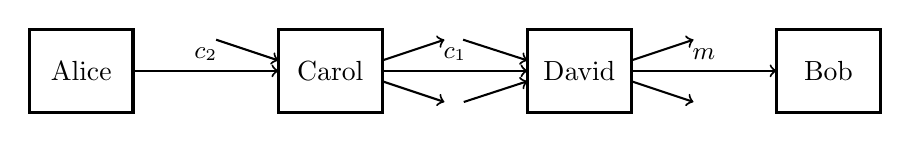
\begin{tikzpicture}[x=0.75pt,y=0.75pt,yscale=-1,xscale=1]

\draw  [line width=1.2] (0,20) -- (50,20) -- (50,60) -- (0,60) -- cycle ;
\draw  [line width=1.2] (120,20) -- (170,20) -- (170,60) -- (120,60) -- cycle ;
\draw  [line width=1.2] (240,20) -- (290,20) -- (290,60) -- (240,60) -- cycle ;
\draw  [line width=1.2] (360,20) -- (410,20) -- (410,60) -- (360,60) -- cycle ;

\draw  [->]  (50,40) -- (120,40) ;
\draw  [->]  (170,40) -- (240,40) ;
\draw  [->]  (290,40) -- (360,40) ;
\draw  [->]  (90,25) -- (120,35) ;
\draw  [->]  (209.33,55) -- (240,45) ;
\draw  [->]  (209,25) -- (240,35) ;
\draw  [->]  (170,35) -- (200,25) ;
\draw  [->]  (290,35) -- (320,25) ;
\draw  [->]  (170,45) -- (200,55) ;
\draw  [->]  (290,45) -- (320,55) ;

\draw (25,40) node   [align=left] {Alice};
\draw (145,40) node   [align=left] {Carol};
\draw (265,40) node   [align=left] {David};
\draw (385,40) node   [align=left] {Bob};
\draw (85,32) node  [font=\small]  {$c_{2}$};
\draw (205,32) node [font=\small]   {$c_{1}$};
\draw (325,32) node [font=\small]   {$m$};

\end{tikzpicture}
	\caption{一个使用两层混合的洋葱路由的例子}
	\label{fig:2-7}
\end{figure}

现在,Carol 就算监测了所有的网络流量,也无法确定谁在 Bob 的论坛上发布了特定的某条消息。这对于 David 来说也是一样。然而,如果 Carol 和 David 是串通的,他们就能搞清楚这些信息。由于这个原因,Alice 可能会通过两个以上的混合网络来传递她的消息。只要其中至少有一个混合服务不与其他服务串谋,Alice 就能够保证她的匿名性。

一个稍微有点复杂的情况是,当 Alice 与 David 建立共享秘钥 $k_{\rm d}$ 时,她不能向 David 透露她的身份。否则,David 就会知道 $c_1$ 来自 Alice,这是我们不希望看到的。这个目标并不难实现,我们将在本书后面介绍如何做到这一点(见 \ref{sec:21-13} 节)。

\begin{snote}[嵌套加密的安全性。]
为了确保 Alice 的匿名性,知道 $k_{\rm c}$ 的 Carol 不能从式 \ref{eq:2-12} 的嵌套密文 $c_2$ 中获取任何关于 $m$ 的信息。否则,Carol 就有可能利用她从 $c_2$ 中了解到的关于 $m$ 的信息,将 Alice 与她在 Bob 的论坛上发的帖子联系起来。比如说,假设 Carol 可以从 $c_2$ 中了解到 $m$ 的前几个字符,然后她发现 Bob 的论坛上只有一个帖子以这些字符开头。那么 Carol 就可以将整个帖子与 Alice 关联起来,因为她知道 $c_2$ 是来自 Alice 的。

对 David 来说,情况也是如此:知道 $k_{\rm d}$ 的 David 最好无法从式 \ref{eq:2-12} 的嵌套密文 $c_2$ 中得知任何关于 $m$ 的信息。

我们下面论证,如果 $\mathcal{E}$ 是语义安全的,那么在给定 $c_2$ 和 $k_c$ 或 $k_d$ 两个密钥中的一个的情况下,任何有效对手都无法了解任何关于 $m$ 的信息。
\end{snote}

一般地,对于一个定义在 $(\mathcal{K},\mathcal{M},\mathcal{C})$ 上的密码 $\mathcal{E}=(E,D)$,我们定义 $n$ 层嵌套密码 $\mathcal{E}_n=(E_n,D_n)$ 如下:
\[
E_n\big((k0,\dots,k_{n-1}),\,m\big)=E\big(k_{n-1},\,E(k_{n-2},\,\cdots E(k_0,m)\cdots\big)
\]
解密算法以相反的顺序使用密钥:
\[
D_n\big((k0,\dots,k_{n-1}),\,c\big)=D\big(k_0,\,E(k_1,\,\cdots E(k_{n-1},m)\cdots\big)
\]
我们的目标是表明,如果 $\mathcal{E}$ 是语义安全的,那么就算对手得到了 $k_0,\dots,k_{n-1}$ 中除某一个之外的所有密钥,$\mathcal{E}_n$ 也是语义安全的。为了更加精确,我们定义两个实验:实验 $0$ 和实验 $1$,对于 $b=0,1$,实验 $b$ 的工作方式如下:
\begin{itemize}
	\item 对手将 $(m_0,m_1,d)$ 交给挑战者,其中 $m_0,m_1\in\mathcal{M}$ 是长度相等的两条消息,且 $0\leq d<n$。
	\item 挑战者选择 $n$ 个密钥 $k_0,\dots,k_{n-1}\overset{\rm R}\leftarrow\mathcal{K}$ 并计算 $c\overset{\rm R}\leftarrow E_n\big((k_0,\dots,k_{n-1}),\,m_b\big)$。它将 $c$ 和所有的密钥 $k_0,\dots,k_{n-1}$ 一起发送给对手,但不包括密钥 $k_{d}$。
	\item 对手输出一个比特 $\hat b\in\{0,1\}$。
\end{itemize}
这个游戏抓住了这样一个事实:对手得到除 $k_{d}$ 以外的所有密钥 $k_0,\dots,k_{n-1}$,并试图破坏语义安全性。

和语义安全性的定义一样,我们将对手的优势 $\mathrm{NE^{(n)}}\mathsf{adv}[\mathcal{A},\mathcal{E}]$ 定义为:
\[
\mathrm{NE^{(n)}}\mathsf{adv}[\mathcal{A},\mathcal{E}]=\big\vert\Pr[W_0]-\Pr[W_1]\big\vert
\]
其中 $W_b$ 是 $\mathcal{A}$ 在实验 $b$ 中输出 $1$ 的事件,对于 $b=0,1$,如果 $\mathrm{NE^{(n)}}\mathsf{adv}[\mathcal{A},\mathcal{E}]$ 可忽略不计,我们就说 $\mathcal{E}$ 对于 $n$ 层嵌套是语义安全的。

\begin{theorem}\label{theo:2-12}
对于每个常数 $n>0$,如果 $\mathcal{E}=(E,D)$ 是语义安全的,那么 $\mathcal{E}$ 对于 $n$ 层嵌套来说也是语义安全的。
\begin{quote}
特别地,对于每个攻击 $\mathcal{E}_n$ 的 $n$ 层嵌套对手 $\mathcal{A}$,都存在一个攻击 $\mathcal{E}$ 的语义安全对手 $\mathcal{B}$,其中 $\mathcal{B}$ 是一个围绕 $\mathcal{A}$ 的基本包装器,满足:
\end{quote}
\[
\mathrm{NE^{(n)}}\mathsf{adv}[\mathcal{A},\mathcal{E}]=\mathrm{SS}\mathsf{adv}[\mathcal{B},\mathcal{E}]
\]
\end{theorem}

\noindent
这个定理的证明很适合作为安全归约的练习。我们将其留作练习 \ref{exer:2-15}。